\chapter{Implementation}

As has been explained before, the implementation should be a .NET library usable from C\#. While it would be possible to write such a library in another .NET language, C\#, as a general-purpose programming language, is suitable for this task, so it is the language used in the implementation.

One of the principles of the design of the system has been a focus on performance, especially when it comes to limiting executing the code of transformations. The implementation also sometimes considers performance, but generally speaking, maintainability and readability of code take precedence, especially at the method level. Because some of the code written this way might be performance-critical, the intention is to use profiling and optimize the found bottlenecks, but this has not been done in the current version.

\medskip

\label{projects}
The implementation of the system is composed of four main projects:

\begin{itemize}
\item \cs{CSharpE.Syntax}, for representing code,
\item \cs{CSharpE.Transform}, for transforming code,
\item \cs{CSharpE.Transform.VisualStudio}, which supports using extensions at design-time in Visual Studio,
\item \cs{CSharpE.Transform.MSBuild}, which supports using extensions at build-time in MSBuild.
\end{itemize}

\section{CSharpE.Syntax}

The most complicated part of the job of \cs{CSharpE.Syntax} is to convert from C\# source code to CSharpE code representation and vice versa. To help with this, we can use Roslyn. Thanks to Roslyn, it is only necessary to write code that converts between the Roslyn representation and the CSharpE representation, which is much easier. Also, by using Roslyn, we use the same code as the C\# compiler, which means there is no chance of introducing parsing bugs.

\medskip

Because CSharpE syntax nodes and Roslyn syntax nodes often have very close correspondence and because transformations often access only some parts of the syntax tree, a CSharpE syntax tree that is created from a Roslyn syntax tree acts as a lazy wrapper over it: CSharpE nodes are created from the corresponding Roslyn nodes only as necessary. In other words, when a CSharpE node is created from a Roslyn node, it stores the Roslyn node. When one of its child nodes is then accessed for the first time, it is created from the corresponding child of the Roslyn node.

Syntax nodes can also have properties that are not child syntax nodes and are not lazy. For example, the property \cs{string Name} of \cs{TypeDefinition} is one.

\medskip

After a CSharpE syntax node is created, it can then be modified by the user. Eventually, it will need to be converted back to C\# source code, which is once more done through Roslyn nodes: CSharpE nodes implement the internal interface \cs{ISyntaxWrapper<TSyntax>}, which can be seen in Listing~\ref{isyntaxwrapper}. The single method of this interface, \cs{GetWrapped}, is used to retrieve an up-to-date version of the Roslyn node (\cs{TSyntax}) for a CSharpE node. The \cs{changed} parameter is used by the \cs{GetWrapped} method of the parent node to detect whether the current node changed since the parent called the \cs{GetWrapped} method of the child node last. Any other caller is required to pass a reference to \cs{null} for the parameter.

\begin{listing}
\begin{minted}{csharp}
internal interface ISyntaxWrapper<out TSyntax>
{
    TSyntax GetWrapped(ref bool? changed);
}
\end{minted}
\caption{Declaration of the ISyntaxWrapper interface}
\label{isyntaxwrapper}
\end{listing}

Another option would be to notify ancestor nodes whenever a node is modified. This way, a node that has not changed would not have to be inspected for changes, which could be more efficient. Though this approach is more complicated and so it has not been implemented.

\medskip

\begin{listing}
\begin{minted}{csharp}
public sealed class Argument : SyntaxNode, ISyntaxWrapper<ArgumentSyntax>
{
    private ArgumentSyntax syntax;

    internal Argument(ArgumentSyntax syntax, SyntaxNode parent)
    {
        this.syntax = syntax ?? throw new ArgumentNullException(nameof(syntax));
        Name = syntax.NameColon?.Name.Identifier.ValueText;
        Parent = parent;
    }

    public Argument(Expression expression, string name = null)
    {
        Expression = expression;
        Name = name;
    }

    public string Name { get; set; }

    private Expression expression;
    public Expression Expression
    {
        get => expression ??
            (expression = FromRoslyn.Expression(syntax.Expression, this));
        set => SetNotNull(ref expression, value);
    }

    ArgumentSyntax ISyntaxWrapper<ArgumentSyntax>.GetWrapped(ref bool? changed)
    {
        GetAndResetChanged(ref changed);
        
        bool? thisChanged = false;
        var newExpression =
            expression?.GetWrapped(ref thisChanged) ?? syntax.Expression;

        if (syntax == null || thisChanged == true ||
            syntax.NameColon?.Name.Identifier.ValueText != Name)
        {
            syntax = RoslynSyntaxFactory.Argument(
                Name == null ? null : CSharpSyntaxFactory.NameColon(Name),
                default, newExpression);

            SetChanged(ref changed);
        }

        return syntax;
    }

    public static implicit operator Argument(Expression expression)
        => new Argument(expression);
}
\end{minted}
\caption{Simplified implementation of the Argument class}
\label{argument-source}
\end{listing}

Listing~\ref{argument-source} shows how a typical implementation of a \cs{SyntaxNode} looks like. Specifically, it shows simplified code of the \cs{Argument} class, which is used to represent an argument to a call. For example, the statement \cs{F(42, foo: null);} contains two arguments: \cs{42} and \cs{foo: null}. An argument is composed of an expression, an optional name and an optional ref kind (\cs{ref}, \cs{out} or \cs{in}). For brevity, the version of \cs{Argument} shown here does not support arguments that have a ref kind. This means that the class has two properties: the lazy \cs{Expression} and the non-lazy \cs{Name}.

The implementation is composed of the following parts:

\begin{itemize}
\item Specification that the class directly inherits from the \cs{SyntaxNode} base class and that it implements the \cs{ISyntaxWrapper<TSyntax>} interface for Roslyn's \cs{ArgumentSyntax} type.

\item A field holding the most recent Roslyn syntax node, if any.

\item An internal constructor that creates an instance of the class from a Roslyn syntax node.

Notice that the lazy property \cs{Expression} is not initialized here, while the non-lazy property \cs{Name} is. Another interesting point is how complicated the expression used to initialize \cs{Name} is, which shows that the CSharpE design is much simpler than the Roslyn design in this case.

This constructor is used when a member of the \cs{Arguments} collection of \cs{InvocationExpression} or a similar kind of expression is accessed for the first time.

\item A public constructor that can be used by the user to create a new instance of this class.

\item The \cs{Name} property.

Because it is not lazy, it does not require any special behavior and so it can be an auto-property.

\item The \cs{Expression} property.

Since it is lazy, when its value is read for the first time, the \cs{Expression} node is created based on the expression of the Roslyn node. The \cs{FromRoslyn} class contains helper methods for converting Roslyn nodes to CSharpE nodes. In this case, it is used to create the correct type that derives from \cs{Expression} based on the Roslyn node.

The setter uses the helper method \cs{SetNotNull}, which checks that the passed in value is not \cs{null} and also ensures that the \cs{Parent} property of the expression node is correctly set. (The \cs{Parent} property is explained in more detail later.)

\item The \cs{GetWrapped} method.

It is an explicit interface implementation, because C\# does not allow implicit interface implementations through internal methods, only public ones, and this method should not be accessible by the user.

The method does the following:

\begin{enumerate}
\item Make sure that the value of the \cs{changed} parameter is set correctly when this method is called by the parent node by invoking the helper methods \cs{GetAndResetChanged} and \cs{SetChanged} at the appropriate places.
\item Call \cs{GetWrapped} on its lazy properties if they are initialized, otherwise use the corresponding child of the saved Roslyn node. While doing this, keep track of whether any lazy properties reported changes in the \cs{thisChanged} variable.
\item Check if a new Roslyn node needs to be created. This happens either because no Roslyn node has been created yet, or because changes occurred since the saved Roslyn node was created. Changes are detected by checking the \cs{thisChanged} variable for lazy properties and by comparing with the latest Roslyn node for non-lazy properties.
\item Create a new Roslyn node by using a factory method from the Roslyn \cs{SyntaxFactory} class (aliased as \cs{RoslynSyntaxFactory} because of a conflict with CSharpE \cs{SyntaxFactory}) and save it.
\item Finally, return the Roslyn node, which is now guaranteed to be up to date.
\end{enumerate}

Note that the returned Roslyn node will have no parent. When the caller is the CSharpE parent node, it will incorporate that Roslyn node into its own Roslyn node, but with parent set to that node. This happens automatically when any Roslyn node with child nodes is created.

To make this efficient, Roslyn uses a data structure called "red-green tree" (unrelated to the well-known red-black tree), where the regular nodes (which have parent references, and so cannot be reused) are a layer on top of hidden nodes with no parent references, which are reused. \cite{red-green-trees}

\item An implicit conversion operator from \cs{Expression} to \cs{Argument}.

\nopagebreak

This way, the common case where an argument has only an expression, without a name or a ref kind, can be created more easily.
\end{itemize}

Other syntax nodes generally follow this pattern, with some exceptions:

\begin{itemize}
\item Accessing any semantic information is more complicated.

As explained in Section~\ref{roslyn}, Roslyn provides semantic information though the \cs{Compilation} and \cs{SemanticModel} classes. For example, to get the full name of a \cs{NamedTypeReference}, such as the type reference \cs{Task} in the field declaration \cs{Task t;}, the following happens:

\begin{enumerate}
\item The \cs{Compilation} for the project is created.

To do that, information from the whole project is necessary, which means that every node that exposes semantic information has to have access to the \cs{Project} object. The way this is done is by making every node have a reference to its parent node. With that, the \cs{SourceFile} that contains a node can be found by recursively walking parent references, and \cs{SourceFile} contains a reference to its \cs{Project}.

\item The \cs{SemanticModel} for the source file is created.

\item A symbol corresponding to the node in question is retrieved from the \cs{SemanticModel}.

This requires using exactly the node that is part of the Roslyn syntax tree that was used to create the \cs{Compilation}. As explained above, the node created by \cs{GetWrapped} is not that: it has no parent node, and so it couldn't possibly be part of the syntax tree.

To find the corresponding node that is part of the syntax tree, we use Roslyn Syntax Annotations. \cite{roslyn-annotations} The Roslyn node returned from \cs{GetWrapped} is annotated with an annotation unique for the current CSharpE node. Then, a node with the same annotation is found in the syntax tree. Finally, that node is used to find the symbol through \cs{SemanticModel}. This works, because incorporating Roslyn node into a parent preserves annotations.

\item The symbol is used to find the desired information.

In this case, that is the full name of the type of the field declaration, which could be (depending on references in the compilation and using directives in the file) for example \cs{System.Threading.Tasks.Task}, \cs{Microsoft.Build.Utilities.Task} or even a type with a name other than \cs{Task} (if the file contains a using alias directive).

\end{enumerate}

\item Lists of syntax nodes have their own set of types.

In the CSharpE \ac{API}, lists of syntax nodes are represented as \cs{IList<T>}. In Roslyn, such lists are either a \cs{SyntaxList<T>} (for lists with no separator, such as members of a class) or a \cs{SeparatedSyntaxList<T>} (for lists that use comma as a separator, such as arguments of a method call).

To bridge this, CSharpE contains a set of internal list types, that also help with maintaining laziness. Such a list contains a collection, where each item can be either a Roslyn node or a CSharpE node. When an item in the list is accessed, it is converted to a CSharpE node, if it is not one already. When \cs{GetWrapped} is called on the list, the result will include Roslyn nodes from the collection directly, while CSharpE nodes have to be converted by invoking their own \cs{GetWrapped}.

\item Exposed collections implement an interface for use in CSharpE.Transform smart loops.

As explained in Section~\ref{smart-loop-collection}, CSharpE.Transform smart loops need to understand the collections they are iterating. For this reason, CSharpE.Syntax collections implement the \cs{ISyntaxCollection<T>} interface. This interface implements the visitor pattern, so that a smart loop can correctly decide how to process the collection.

\item Whitespace from user code is not preserved.

When a syntax node is created using the Roslyn \cs{SyntaxFactory}, it contains so called "elastic trivia", which is meant to be later replaced with proper trivia based on some formatting conventions. But if this step is not performed and the node is converted to a string, the result is invalid code. For example, \cs{SyntaxFactory.ClassDeclaration("Foo").ToString()} returns \cs{classFoo{}}, which is not valid C\# code, because there is nothing separating the tokens \cs{class} and \cs{Foo}.

The easiest way to fix this is to call \cs{NormalizeWhitespace()}, though using that has the side-effect of reformatting all code, including code originally written by the user. But because the user is only ever going to see the reformatted code when debugging (as explained in Section~\ref{debugging}), this was considered an acceptable solution.
\end{itemize}

\section{CSharpE.Transform}

Now that types necessary for representing and modifying code have been implemented, it is time to turn to code that will drive transformations. \label{ProjectTransformer} While Section~\ref{transform-design} described the user-facing \ac{API} of CSharpE.Transform, there is one more public type, \cs{ProjectTransformer}, which is used by the Visual Studio and MSBuild extensions to run transformations. To isolate this type from user-facing types, it is placed in a separate namespace: \cs{CSharpE.Transform.Execution}.

\begin{listing}
\begin{minted}{csharp}
public class ProjectTransformer
{
    public ProjectTransformer(
        IEnumerable<ITransformation> transformations, bool designTime);

    public event Action<LogAction> Log;

    public Project Transform(Project project);
}
\end{minted}
\caption{API of the ProjectTransformer class}
\label{projecttransformer-source}
\end{listing}

Listing~\ref{projecttransformer-source} shows the \ac{API} of \cs{ProjectTransformer}. An instance of this class is created by specifying a collection of transformations and whether they should be executed in design-time or build-time mode. Next, we can subscribe to the \cs{Log} event to diagnose how transformations are executed, as we have seen in Listing~\ref{csharpetransform-log}. (Note that this event does not follow the recommended pattern of using the \cs{EventHandler<T>} delegate. \cite{fdg-events} The approach used here is simpler and is sufficient for the purpose of subscribing to diagnostic information.) Finally, the \cs{Transform} method is used to execute the transformations on the specified project.

The \cs{Transform} method can be called repeatedly to keep executing the same transformations. If it is called for a project that contains code similar to previous project, results of transformations will be retrieved from caches, making the process more efficient.

Even though \cs{Project} is mutable, the method does not modify its input and instead returns a new \cs{Project} instance. This is done so that the caller can keep modifying the original project after the transformation is performed.

\medskip

When a \cs{ProjectTransformer} is created, it creates a \cs{CodeTransformer} for each transformation. \cs{CodeTransformer} handles efficiently executing that transformation. When the \cs{Transform} method is called, a \cs{TransformProject} is created for the input project, then each \cs{CodeTransformer} is applied to it.

\cs{TransformProject} is a type that inherits from \cs{Project}, with some additions in support of executing transformations.

\medskip

\cs{CodeTransformer<TInput, TOutput>} is used to execute a piece of user code, which mutates its input and optionally also returns output. If the piece of code executed within a \cs{CodeTransformer} has no output, unit type (i.e.\ type with no data and only one value) is used for the \cs{TOutput} type parameter. But because .NET does not have a built-in unit type, and because this unit type does not have to be visible in the \ac{API} of the library, a custom internal type called \cs{Unit} is used.\footnotemark{}

\footnotetext{The \cs{ValueTuple} family of types, which were added to .NET to support C\# tuples, includes the non-generic \cs{ValueTuple} type, representing a tuple with zero elements, even though there is currently no support for zero-element tuples in C\#. This type could be used as a unit type, but a custom type with the name \cs{Unit} makes the intention clearer.}

% While the user code is executing, smart loops and segments have access to information from their previous execution within this \cs{CodeTransformer}, which means they can take advantage of caching. This is done by attaching information about the previous executions to \cs{TransformProject}. Since smart loops and segments always have access to a \cs{Project}, they can detect whether it is a \cs{TransformProject} and act accordingly.

If the input of a \cs{CodeTransformer} is a syntax node, it, or rather, its derived class, \cs{SyntaxNodeCodeTransformer<TInput, TOutput>}, employs caching: When it is detected that the current input is equivalent to the previous input, changes from the previous input are directly applied to the current one, without recomputing them. Because there are variations to this process, it is represented as a delegate of the type \cs{Func<T, Func<Action<T>>>}, which is somewhat similar to the curried form of a function type in functional programming. This delegate shape is used here, because the delegate is invoked in three stages, each at a different point in the process of executing the user code: the first stage is invoked before the code is executed (and is provided with the input syntax node), the second stage is invoked after the code is executed (and does not have input of its own, because all it needs is the syntax node, which was already provided in the previous stage and has been mutated since then), and the third stage can be repeatedly invoked whenever there is a next equivalent input (and is provided with that input).

Specifically, the variations of this delegate are:

\begin{itemize}
\item Regular.

For most user code, the "before" stage does nothing, syntax is retrieved from the input during the "after" stage (by calling \cs{GetWrapped} on it) and the input of the "next" stage is mutated by forcing this syntax into it.

\item Smart segment.

User code that executes within a smart segment requires special handling. The only valid changes within such segment are adding new members. This means that if the delegate only preserves these new members, the concept of equivalence can be broadened, resulting in more cache hits.

To do this, the number of members of the input is recorded in the "before" stage, then members above this count are saved in the "after" stage, and finally, these members are added to the input of the "next" stage.

\item Using directives.

The code that executes within a \cs{SyntaxNodeCodeTransformer} is not allowed to modify syntax outside of its input, with one exception: \cs{using} directives. When newly added syntax nodes reference a type from a name\-space that does not have a \cs{using} directive in the file yet, CSharpE adds the directive automatically. But this has to be replicated also when those syntax nodes are being added from a cache. For this purpose, \cs{SourceFile} includes functionality to record requests to ensure a \cs{using} directive exists.

In the "before" stage, this recording is started on the input, in the "after" stage, recording is stopped and its results retrieved and for the input of the "next" stage, the recorded namespaces are requested again. This happens on top of one of the two delegates described above.
\end{itemize}

This caching is at the core of ensuring that user code is not executed unnecessarily in CSharpE.Transform and it is what each "cached" line in Listing~\ref{csharpetransform-log} represents. But to make this work, each \cs{CodeTransformer} also has to maintain information about the execution of smart loops and segments within it.

\medskip

This information is kept in a list of objects of type \cs{CollectionTransformer}. When a smart loop or segment is invoked within user code, information about it is matched against an object from the list. If the match is successful, the old object is reused, otherwise, new \cs{CollectionTransformer} is created.

Since the user code in question is always the same, it is expected that it will usually invoke the same smart loops and segments when it is executed, which should result in high levels of reuse of \cs{CollectionTransformer} objects.

Specifically, each object in the list is a \cs{CollectionTransformer<TParent, TItem, TData, TIntermediate, TResult>}. The meaning of the type parameters for a smart loop is:

\begin{itemize}
\item \cs{TParent} is the type that contains the collection.
\item \cs{TItem} is the type of items in the collection.
\item \cs{TData} is the type of data that is used as input for user code.
\item \cs{TIntermediate} is the result type of each iteration of the smart loop.
\item \cs{TResult} is the result type of the whole smart loop.
\end{itemize}

\pagebreak[2]

A smart segment behaves in many respects like a smart loop over a collection with a single element. This means that for example both \cs{TParent} and \cs{TItem} are \cs{TypeDefinition} for them. Another case where some of the type parameters are effectively unused is for smart loops that do no return a value: in that case, both \cs{TIntermediate} and \cs{TResult} are \cs{Unit}.

To further clarify the meaning of the type parameters, consider the following example code, modified from Listing~\ref{csharpetransform-smart-example2}:

\begin{minted}{csharp}
var fieldsList = Smart.ForEach(classDefinition.Fields, classDefinition.Name,
    (className, field) => (className, field.Type, field.Name));
\end{minted}

The \cs{CollectionTransformer} used for this code has the following type parameters:

\bigskip \noindent
\begin{tabular}{ll}
Type parameter     & Value \\
\midrule
\cs{TParent}       & \cs{SyntaxNode} (for \cs{classDefinition}) \\
\cs{TItem}         & \cs{FieldDefinition} \\
\cs{TData}         & \cs{string} (for \cs{classDefinition.Name}) \\
\cs{TIntermediate} & \cs{(string, TypeReference, string)} \\
\cs{TResult}       & \cs{List<(string, TypeReference, string)>}
\end{tabular}

\bigskip

What the implementation of \cs{CollectionTransformer} actually does is that it maintains \cs{CodeTransformer} objects and whenever it processes a collection, it reuses one of these objects, if it matches the item that is currently being processed. There are two variants of \cs{CollectionTransformer} and each of them does this differently:

\begin{itemize}
\item \cs{SourceFileCollectionTransformer} is used when processing source files in a project. Files are considered to match when they have the same path (including file name).
\item \cs{SyntaxNodeCollectionTransformer} is used when processing syntax nodes within a file. Syntax nodes are considered to match based on a diff of the parent node. This way, when some nodes are added to or removed from the collection, the remaining nodes (including those that were changed) should still have their \cs{CodeTransformer} reused.
\end{itemize}

In both cases, when \cs{CodeTransformer} objects are reused, it means that their matching comes into effect, which can lead to avoiding rerunning the relevant piece of user code, thanks to caching.

\section{CSharpE.Transform.MSBuild}

Now that CSharpE.Transform has been implemented, it is time to use it. First, we create an MSBuild \cs{Task} to support executing build-time transformations from \acp{IDE} or from the command line. MSBuild has variants for both .NET Framework and .NET Core and both will need to be capable of running this \cs{Task}, because the .NET Framework variant is used by Visual Studio and the .NET Core variant is required by Linux build servers. This means that the \cs{Task} will have to be capable of running on both frameworks.

The \cs{Task} will need to load referenced extension assemblies to execute the transformations contained within them. To avoid issues with assembly loading we could take advantage of assembly isolation (\cs{AppDomain} in .NET Framework and \cs{AssemblyLoadContext} in .NET Core) either directly or by using a library, \cite{nb-msbe} but this approach does not seem to be reliable. So, a separate process is used instead.

The way it works is that the assembly with the \cs{Task} is loaded as a regular MSBuild extension library. It then relaunches itself as an application, which actually executes the transformations. The two processes communicate with each other using a rudimentary text-based protocol: the MSBuild extension writes paths of references (including references to CSharpE extensions) and input source files to the standard input of the second process and then reads warnings, errors and paths of transformed source files from its standard output.

\medskip

The MSBuild process is generally not reused between builds, which means this approach will always execute full transformations, with no caching. This is acceptable, because building is not particularly performance sensitive, certainly significantly less sensitive than \ac{IDE} operations like autocompletion.

MSBuild \cs{Task}s are usually executed not just during regular build, but also during "design-time build". \cite{design-time-builds} Because such builds are used by \acp{IDE}, but CSharpE requires special handling for those, the \cs{Task} described in this section specifically does not execute during design-time builds.

\section{CSharpE.Transform.VisualStudio}

After support for MSBuild, the next step is to add support for the Visual Studio \ac{IDE}. Most of the support in Visual Studio for C\# comes from a Visual Studio extension that is open source and part of the Roslyn project, but this support is not useful for CSharpE on its own, because it has no knowledge of CSharpE transformations. Possible approaches to make this work are:

\begin{enumerate}
\item Attempt to extend the C\# extension, so that it also supports CSharpE.
\item Improve the C\# extension to make it more suitable for extending to support CSharpE.
\item Modify the C\# extension to support CSharpE, by creating a fork of Roslyn.
\item Implement support for CSharpE from scratch, without using the existing support for C\#.
\end{enumerate}

Option 1 looks promising  at first: Visual Studio and the C\# extension use \ac{MEF} for their components, which means it could be possible to replace the C\# components with CSharpE components.

Specifically, this can be accomplished thanks to the way the C\# extension uses \ac{MEF}. When the relevant components are resolved, only the one with the highest \cs{ServiceLayer} is selected. This means that CSharpE components will be chosen, if they specify higher \cs{ServiceLayer} than the corresponding C\# components.

Another question is: which components to replace? For example, the Roslyn \ac{API} contains the abstract class \cs{CompletionService}. Creating a class that derives from it allows specifying which items show in code completion. But there is no such component that would allow overriding which errors and warnings show in the Error List, which is necessary to make CSharpE work well in Visual Studio.

Roslyn also contains more low-level services: \cs{ISyntaxTreeFactoryService} and \cs{ICompilationFactoryService}, that allow using custom \cs{SyntaxTree} and \cs{Compilation} objects. Overriding those should be enough; unfortunately, they are internal.

Though all is not lost: .NET includes support for the undocumented attribute \cs{IgnoresAccessChecksToAttribute}. \cite{iacta} Applying this attribute is enough for run-time, but because the C\# compiler does not understand the attribute, more work is necessary at compile-time. That work can be done by an MSBuild task, which rewrites referenced assemblies by changing internal members to public ones.\footnotemark \cite{iactg}

\footnotetext{At first sight, this might look like a good opportunity to use CSharpE. But CSharpE is designed for rewriting source code written by the user, not rewriting referenced assemblies. Doing that requires manipulating metadata, not source code, which is why CSharpE is not useful for this purpose. The referenced project uses Mono.Cecil for its metadata manipulation.}

The big issue with this approach is that it leads to code that is likely going to be extremely brittle: Whenever the C\# extension is updated (which usually happens with every minor version of Visual Studio), there is a high chance that it will break the CSharpE extension, because it relies on internal implementation details, which are subject to change.

\medskip

Option 2 is an attempt to make Option 1 less brittle: if the public extensibility points offered by the C\# extension were expanded to support the needs of CSharpE, the chance that an update to the C\# extension would break the CSharpE extension would be significantly diminished. The issue with this option is that it requires cooperation from the maintainers of the C\# extension, which is uncertain.

\medskip

Option 3 would be to create a version of the C\# extension with support for CSharpE, instead of building the CSharpE extension on top of the C\# extension. Doing this would require creating and maintaining a fork of the Roslyn repository. The advantage, compared with Option 1, is that there would be no need to use problematic techniques like \cs{IgnoresAccessChecksToAttribute}. The disadvantage is that this could make the CSharpE extension even more brittle with respect to changes in Roslyn: a change in Roslyn that would not affect Option 1 could still cause a merge conflict with this approach.

\medskip

Option 4 is to create an extension for CSharpE that is largely independent of the C\# extension, though it could reuse some of its services. This approach avoids the brittleness issues of Options 1 and 3 and the dependency on maintainers of Roslyn of Option 2. But it would likely require a significant amount of work to reimplement all the necessary services and the end result would probably still not be on a par with what is offered by the C\# extension.

\medskip

For the long-term health of the CSharpE project, Option 2 would be ideal. If that proved infeasible, then Option 4 might become necessary. But because this is currently only a short-term project, Option 1 was chosen instead.

What this means is that the Visual Studio extension for CSharpE implements \cs{ISyntaxTreeFactoryService} and \cs{ICompilationFactoryService} in such a way that they override their C\# versions. These services are used to provide custom implementations of \cs{SyntaxTree}, \cs{Compilation} and \cs{SemanticModel}. All of these generally delegate to their C\# versions, except that syntax nodes and file locations often have to be mapped back and forth between the original source code and source code after all design-time transformations have been run.

For mapping between nodes, Roslyn Syntax Annotations are used: nodes in original trees are annotated before transformations are run. Then, if semantic information about a node is requested, a node with the same annotation in the corresponding transformed tree is located and its information is returned instead. Since a transformation can remove or replace nodes, this process can fail, with no information being returned.

For mapping between source file locations, annotations are not fine-grained enough, so diffs are used instead. Roslyn contains the \cs{SyntaxDiffer} class for computing diffs between syntax trees, but this was insufficient. Because of that, an enhanced copy of this class is used.

\medskip

The core of the CSharpE Visual Studio extension is in its implementation of \cs{Compilation}: it contains the original C\# \cs{Compilation} and also a lazily computed C\# \cs{Compilation} containing code with design-time transformations applied. These two \cs{Compilation}s are then used as appropriate to implement the required \cs{abstract} methods. \cs{ProjectTransformer}, described in Section~\ref{ProjectTransformer}, is used to compute the compilation with transformations applied. Because the \cs{Compilation} class is immutable and considered thread-safe, a single instance of \cs{ProjectTransfomer} is used under a mutex for successive modified instances of \cs{Compilation}, so that transformations of code that hasn't changed do not have to be recomputed. One exception is when these modifications include changes to references: a new instance of \cs{ProjectTransformer} is used in that situation, in case a modified reference included a transformation, because \cs{ProjectTransformer} operates on a fixed set of transformations.

\medskip

When a project that uses CSharpE is executed within the Visual Studio Debugger, the code that is displayed to the user is the one produced by MSBuild, which means it is the user code, after performing build-time transformations. So, the code shown to the user is the code that is actually executing, which is especially useful when developing a transformation or when debugging an issue related to the used transformations.

At the same time, a transformation can introduce a large amount of "boilerplate code" (which is one of the main reasons why transformations are useful in the first place), and this additional code can hamper understanding how the user code executes. While this means that some kind of simplified debugging view could be useful, it has not been implemented.

\medskip

\begin{figure}[p]
\centering
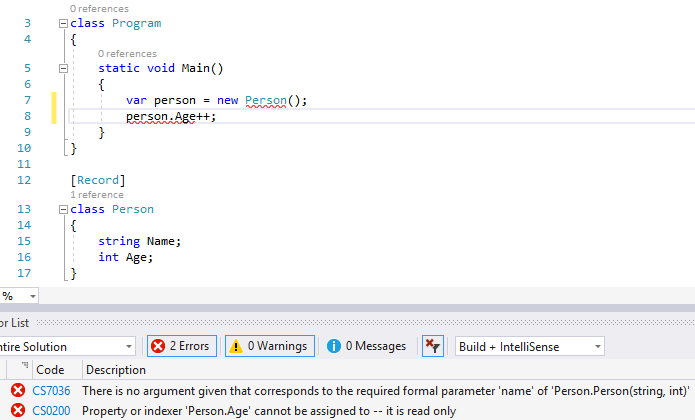
\includegraphics[width=\textwidth]{errors}
\caption{Example of error reporting}
\label{figure-errors}
\end{figure}

\begin{figure}[p]
\centering
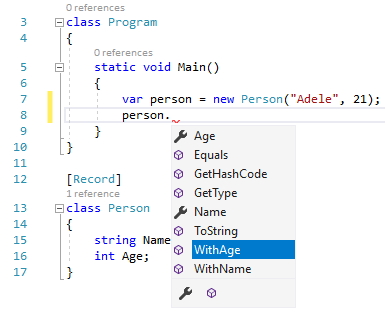
\includegraphics{intellisense}
\caption{Example of autocompletion}
\label{figure-intellisense}
\end{figure}

\begin{figure}[p]
\centering
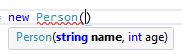
\includegraphics{parameterinfo}
\caption{Example of parameter info}
\label{figure-parameterinfo}
\end{figure}

\begin{figure}[p]
\centering
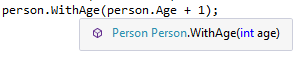
\includegraphics{quickinfo}
\caption{Example of QuickInfo}
\label{figure-quickinfo}
\end{figure}

Figures \ref{figure-errors}, \ref{figure-intellisense}, \ref{figure-parameterinfo} and \ref{figure-quickinfo} show how a very simple CSharpE extension for creating immutable records works in Visual Studio. What the extension does is that it takes a class marked with an attribute and containing some fields and turns it into a proper immutable record with a constructor, read-only properties and \cs{With} methods for creating modified instances. The figures show that Visual Studio features work using CSharpE semantics, not C\# semantics. For example, notice that invoking the parameterless constructor produces an error, while invoking the constructor with parameters corresponding to fields does not. This is the opposite of what would happen in regular C\#.

\medskip

\todo{Conclusion?}

\section{Example extensions}
\label{example-extensions}
